\documentclass[crop,tikz]{standalone}% 'crop' is the default for v1.0, before it was 'preview'
%\usetikzlibrary{...}% tikz package already loaded by 'tikz' option
\begin{document}
  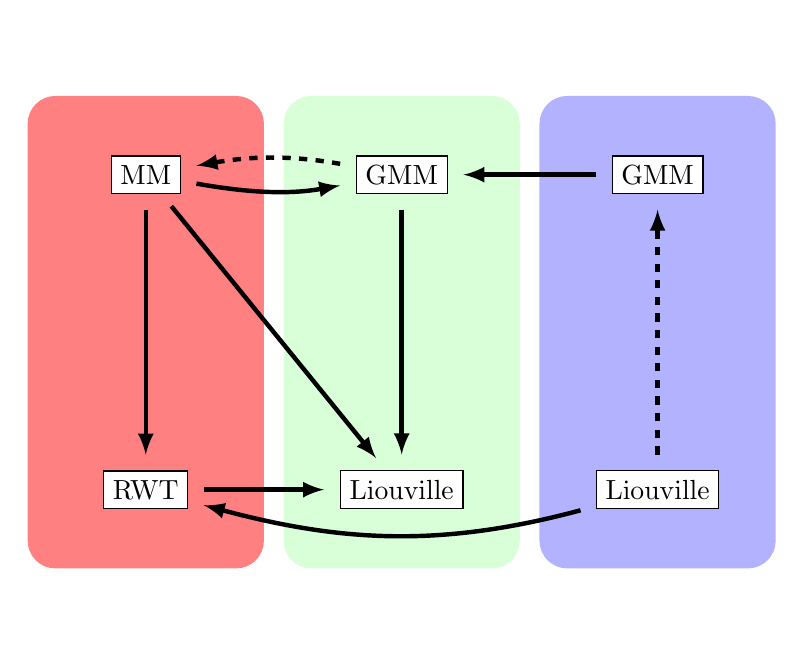
\begin{tikzpicture}[scale = .25]
  \node at (0, 15) {};
  \node at (0, -15){};
\fill[red!50, rounded corners = 10] (-6, -12) rectangle (6, 12);
\fill[green!15, rounded corners = 10] (7, -12) rectangle (19, 12);
\fill[blue!30, rounded corners = 10] (20, -12) rectangle (32, 12);
\draw (0, 8) node[draw, fill = white] (mm) {MM};
\draw (13, 8) node[draw, fill = white] (gmm1) {GMM};
\draw (26, 8) node[draw, fill = white] (gmm2) {GMM};
\draw (0, -8) node[draw, fill = white] (rwt) {RWT};
\draw (13, -8) node[draw, fill = white] (clo) {Liouville};
\draw (26, -8) node[draw, fill = white] (liou) {Liouville};
\draw [ultra thick, shorten <= 2mm, shorten >= 2mm, -latex, 
       out = -10, in = -170] (mm) to (gmm1);
\draw [ultra thick, shorten <= 2mm, shorten >= 2mm, -latex, dashed,
       out = 170, in = 10] (gmm1) to (mm);
\draw [ultra thick, shorten <= 2mm, shorten >= 2mm, -latex] (gmm2) to (gmm1);
\draw [ultra thick, shorten <= 2mm, shorten >= 2mm, -latex] (mm) to (clo);
\draw [ultra thick, shorten <= 2mm, shorten >= 2mm, -latex] (mm) to (rwt);
\draw [ultra thick, shorten <= 2mm, shorten >= 2mm, -latex] (rwt) to (clo);
\draw [ultra thick, shorten <= 2mm, shorten >= 2mm, -latex] (gmm1) to (clo);
\draw [ultra thick, shorten <= 2mm, shorten >= 2mm, -latex,
       out = -165, in = -15] (liou) to (rwt);
\draw [ultra thick, shorten <= 2mm, shorten >= 2mm, -latex, dashed] (liou) to (gmm2);
\end{tikzpicture}
\end{document}
